\section{Results}
\subsection{Initial Code, Importance Sampling, and Statistical Analysis}
For the simulations a highest learning-rate value of $\gamma = 0.4$ was chosen based on recommendations in \cite{Marsland}.
Figure \ref{fig:naive-nin} along with table \ref{tab:naive-nin} shows that the neural network tends to converge faster when the learning rate is increased,
and stays stable at the ground state, when using brute force metropolis sampling. $\gamma = 0.4$ is clearly the best learning rate of the tested ones.
For importance sampling (figure \ref{fig:importance-nin-gamma}, table \ref{tab:importance-nin-gamma})
the data follows the same trend. With importance sampling the precision is lower than that of brute
force metropolis, but the mean variance is lower.
For the best converging value of gamma, a simulation with the same parameters, but varying the
timestep $dt$ was done (figure \ref{fig:importance-nin-dt}, table \ref{tab:importance-nin-dt}).
From the figure and data in the table, the $dt$ parameter influences mainly the variance,
lowering it by $~\frac{1}{3}$ per order of magnitude.

\begin{figure}[h]
\hspace{-2.8cm}
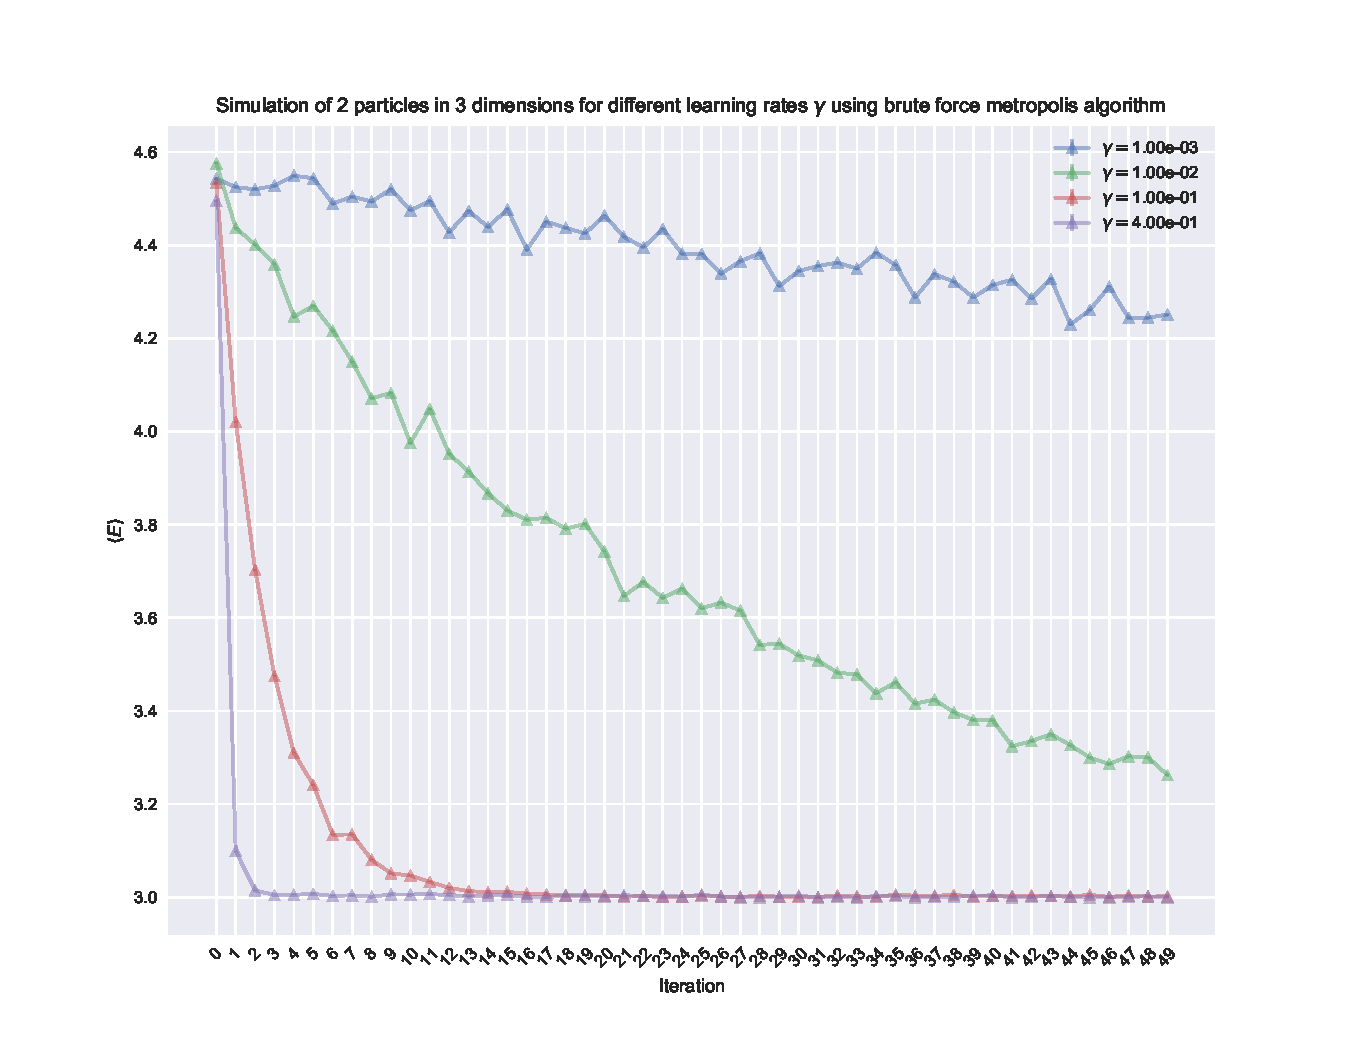
\includegraphics[width = \paperwidth]{figures/naive_2p_3d.pdf}
\caption{Plot of simulation with 2 particles in 3 dimensions with varied learning rates $\gamma$, using brute force metropolis sampling.
			2 hidden nodes were used.
			For detailed values on energy, variance, and CPU-time per mc-cycle, see table \ref{tab:naive-nin}}
\label{fig:naive-nin}
\end{figure}

\begin{table}[h]
\begin{tabular}{l c c}
	Mean time per mc-cycle & &$5.88\cdot10^{-5}$ s \\
	\hline
	$\gamma$ & Mean $\expect{E_L}$ a.u & Mean Variance $\sqrt{\sigma}$\\
	\hline
	$1\cdot10^{-3}$ & $4.36$ & $3.07\cdot10^{-2}$ \\
	$1\cdot10^{-2}$ & $3.57$ & $1.97\cdot10^{-2}$ \\
	$1\cdot10^{-1}$ & $3.005$ & $1.97\cdot10^{-3}$ \\
	$4\cdot10^{-1}$ & $3.002$ & $1.45\cdot10^{-3}$ \\
\end{tabular}
\label{tab:naive-nin}
\caption{Table of learning rates $\gamma$ and mean expectation values for the local energy $E_L$ with mean variance, for brute force metropolis sampling
		of 2 particles in 3 dimensions, with 4 hidden nodes.
		Mean CPU-time per monte-carlo cycle across all iterations at the top.
	For corresponding plot, see figure \ref{fig:naive-nin}}
\end{table}

\begin{figure}[h]
\hspace{-2.8cm}
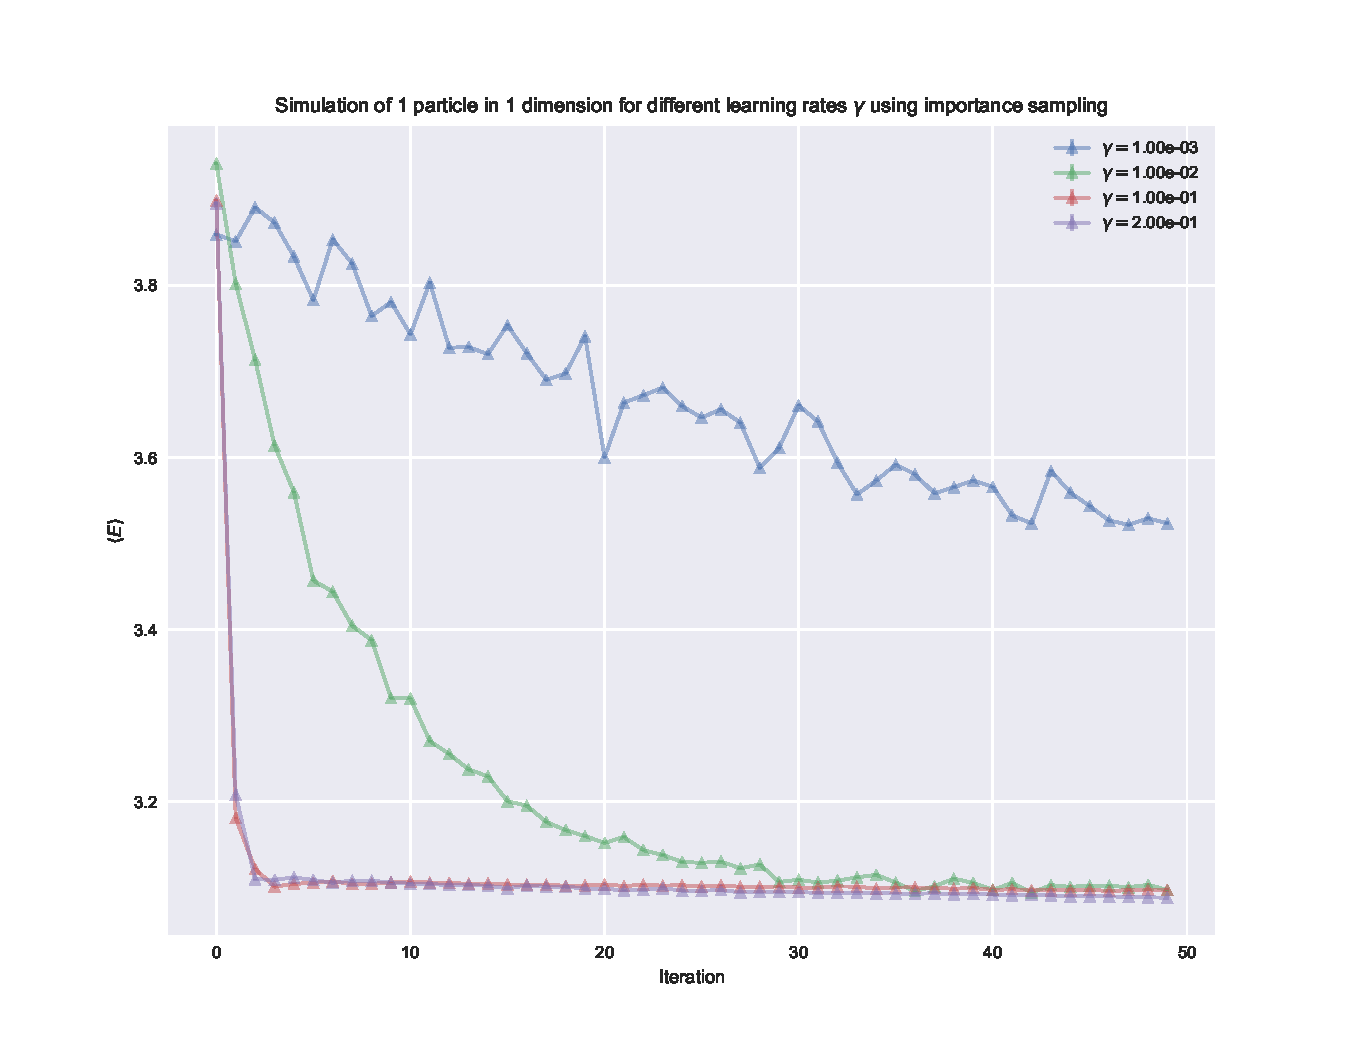
\includegraphics[width = \paperwidth]{figures/importance_2p_3d.pdf}
\caption{Plot of simulation with 2 particles in 3 dimensions with varied learning rates $\gamma$, using brute force metropolis sampling.
			For detailed values on energy, variance, and CPU-time per mc-cycle, see table \ref{tab:importance-nin-gamma}}
\label{fig:importance-nin-gamma}
\end{figure}

\begin{table}[h]
\begin{tabular}{l c c}
	Mean time per mc-cycle & &$5.80\cdot10^{-4}$ s \\
	\hline
	$\gamma$ & $\expect{E_L}$ a.u & Mean Variance $\sqrt{\sigma}$\\
	\hline
	$1\cdot10^{-3}$ & $3.62$ & $2.16\cdot10^{-2}$ \\
	$1\cdot10^{-2}$ & $3.149$ & $6.09\cdot10^{-3}$ \\
	$1\cdot10^{-1}$ & $3.1011$ & $7.51\cdot10^{-4}$ \\
	$2\cdot10^{-1}$ & $3.0959$ & $6.91\cdot10^{-4}$ \\
\end{tabular}
\label{tab:importance-nin-gamma}
\caption{Table of learning rates $\gamma$ and corresponding expectation values obtained for the local energy $E_L$ with variance, for importance sampling
		of 2 particles in 3 dimensions, with 4 hidden nodes.
		Mean CPU-time per monte-carlo cycle across all iterations at the top. 4 hidden nodes were used.
	For corresponding plot, see figure \ref{fig:importance-nin-gamma}}
\end{table}

\begin{figure}[h]
\hspace{-2.8cm}
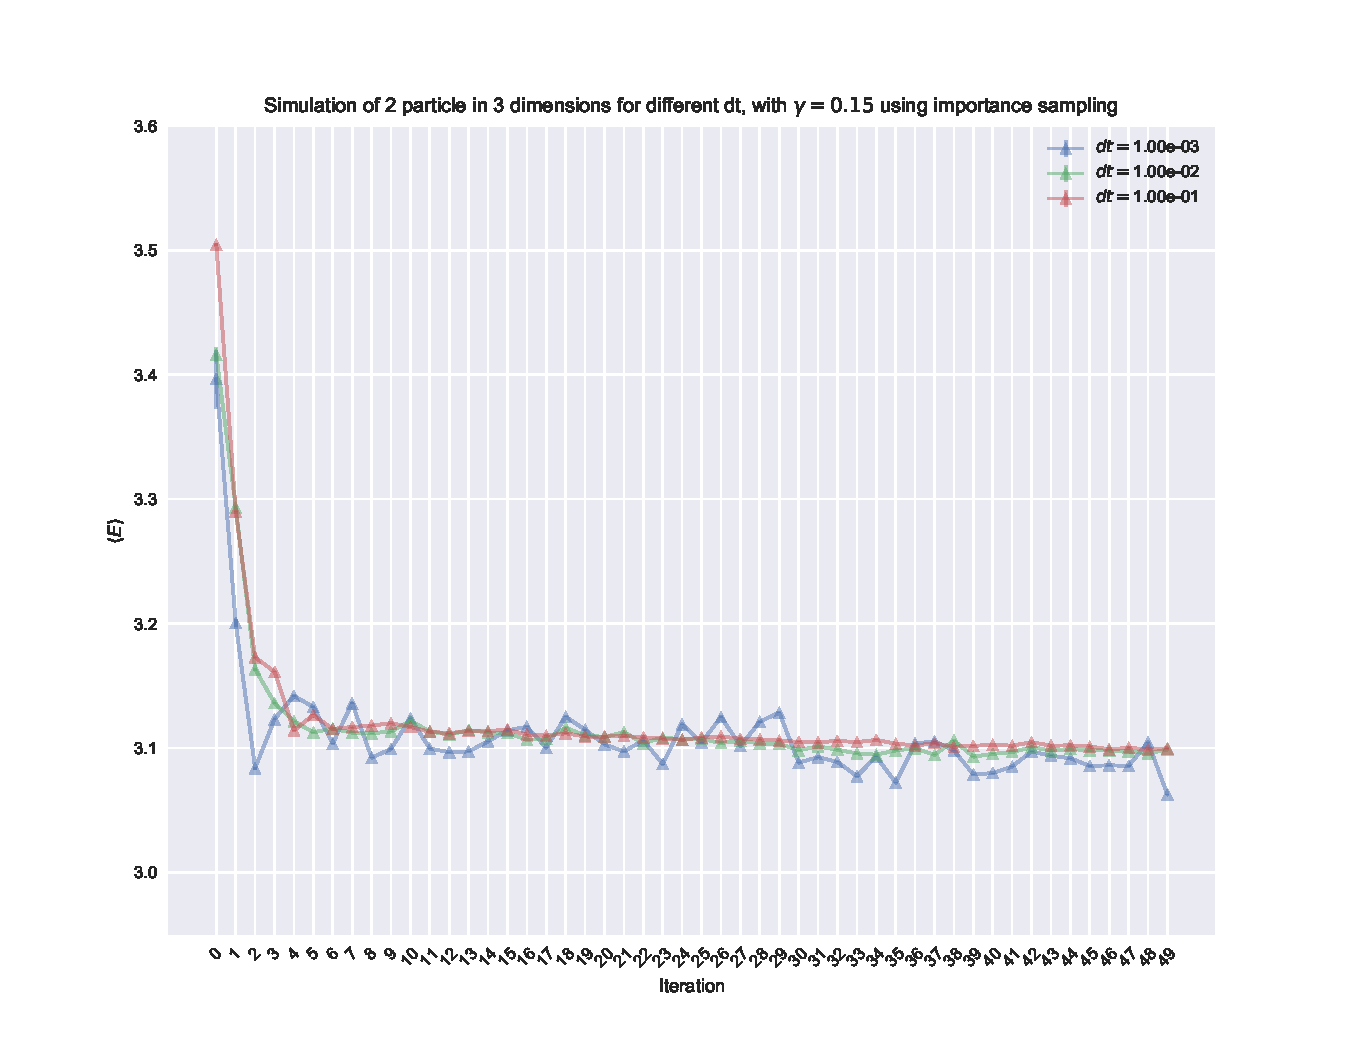
\includegraphics[width = \paperwidth]{figures/importance_2p_3d_dt.pdf}
\caption{Plot of simulation with 2 particles in 3 dimensions with varied learning rates $\gamma$, using brute force metropolis sampling.
			For detailed values on energy, variance, and CPU-time per mc-cycle, see table \ref{tab:importance-nin-dt}}
\label{fig:importance-nin-dt}
\end{figure}

\begin{table}[h]
\begin{tabular}{l c c}
	Mean time per mc-cycle & & $5.24\cdot10^{-4}$ s \\
	\hline
	$dt$ & $\expect{E_L}$ a.u & Mean Variance $\sqrt{\sigma}$\\
	\hline
	$1\cdot10^{-3}$ & $3.099$ & $9.18\cdot10^{-3}$ \\
	$1\cdot10^{-2}$ & $3.103$ & $3.43\cdot10^{-3}$ \\
	$1\cdot10^{-1}$ & $3.106$ & $1.13\cdot10^{-3}$ \\
\end{tabular}
\label{tab:importance-nin-dt}
\caption{Table of timesteps $dt$ and corresponding expectation values obtained for the local energy $E_L$ with variance, for importance sampling
		of 2 particles in 3 dimensions, with 4 hidden nodes.
		Mean CPU-time per monte-carlo cycle across all iterations at the top.
	For corresponding plot, see figure \ref{fig:importance-nin-dt}}
\end{table}

